\section{Variables Cataclísmicas}
Nuestra Galaxia es el hogar de varios sistemas solares, los cuales muestran una
gran variedad de propiedades físicas. Existen sistemas tal como nuestro sistema
solar, que consisten de una estrella de secuencia principal rodeada de planetas
y restos de material de su etapa de formación. Otros sistemas están compuestos
de dos estrellas o más, donde todas las estrellas del sistema orbitan un punto
en común denominado el \textit{centro de masas}. Esta tesis se enfoca en un tipo
de sistema en especifico denominado como \textbf{variables cataclísmicas}:
sistemas de contacto que consisten de una estrella de tipo
\hyperref[intro:sec:EnanaBlanca]{enana blanca} y una
\hyperref[intro:sec:EnanaRoja]{enana roja}. 

\comment{
Este tipo de sistemas muestran comportamiento variable a lo largo del tiempo, en
donde varía su luminosidad, espectro emitido, y otras propiedades del sistema.
No todas las variables cataclísmicas demuestran un comportamiento uniforme; sus
periodos de intensa actividad y el subsecuente periodo de atenuación pueden
variar en su duración y su magnitud. El mecanismo que genera esta variación se
les conoce como \textit{novae}; estos estallidos ocurren debido a la interacción
de las estrellas dentro del sistema.
}

\comment{
\subsection*{Composición de las VCs}
La composición de las estrellas puede variar de un sistema a otro, pero en
general adhieren a los siguientes parámetros: una estrella enana blanca -
conocida como la estrella principal - y una estrella de secuencia principal
menos densa - la estrella secundaria. Esta estrella secundaria es más roja que
la principal; su espectro de emisión tiende a la región roja, llegando hasta el
infra-rojo en ciertos casos. Tomando en cuenta el sistema completo, se puede
observar en la distribución de variables cataclísmicas en el diagrama
Hertzsprung-Russell que la mayoría reside entre las regiones de enanas blancas y
la secuencia principal dependiendo de la contribución relativa de sus estrellas
componentes. \citet{disentanglingGaiaHR} No siempre ocurre algún tipo de
interacción entre las estrellas componentes dentro del sistema; esto va a
depender de los volúmenes de las estrellas y la distancia entre ellas, ya que la
manera principal en que interactúan entre si es en base a su atracción
gravitacional. Entre más cerca de una a otra las fuerzas gravitacionales
empiezan a distorsionar la secundaria hasta tener una forma más plana y menos
uniforme. Este volumen, llamado el lóbulo de Roche, es la región de espacio en
donde la estrella puede mantener a su material atrapada por su gravedad. En un
sistema binario cada estrella tiene un lóbulo de Roche definido, los cuales
están en contacto uno con el otro. Un ejemplo simple se puede ver en la figura
\ref{acrecionSmithReview}, donde la estrella secundaria ha llenado su volumen y
su material empieza a caer hacia la enana blanca debido a su atracción
gravitacional. \\\newline
Al cruzar el lóbulo de Roche de la estrella secundaria, la materia perdida no
puede caer directo a la superficie de la enana blanca a ser absorbida
inmediatamente. Esto se debe al momento angular de las estrellas, tanto por su
rotación como su órbita alrededor de su estrella compañera. Por lo tanto, al
cruzar el punto de contacto entre los lóbulos (este conocido como el punto
Lagrangiano L1) el material tiene una componente de velocidad tangente a la
dirección a la enana blanca. A lo largo de que el material se empieza a acumular
toma una forma dependiendo de las propiedades magnéticas de la enana blanca. En
un sistema donde no ejerce un efecto significativo un campo magnético, el
material forma un \textit{disco de acreción} alrededor de la enana blanca. Este
disco se concentra en el ecuador de esta misma estrella, el cual empieza a
emitir radiación en forma de líneas de emisión. Al contrario en un sistema
magnético (llamados \textit{variables cataclísmicas magnéticas} o
\textit{polares}) donde el campo magnético de la enana blanca es significativo
el material no logra acumularse en un solo disco. Este material debido a ser un
plasma ionizado tiene una carga eléctrica intrínseca, la cual la permite ser
guiada por el campo magnético de la enana blanca a su destino final al polo
magnético de esta misma estrella. \\\newline
\begin{figure}
	\centering
	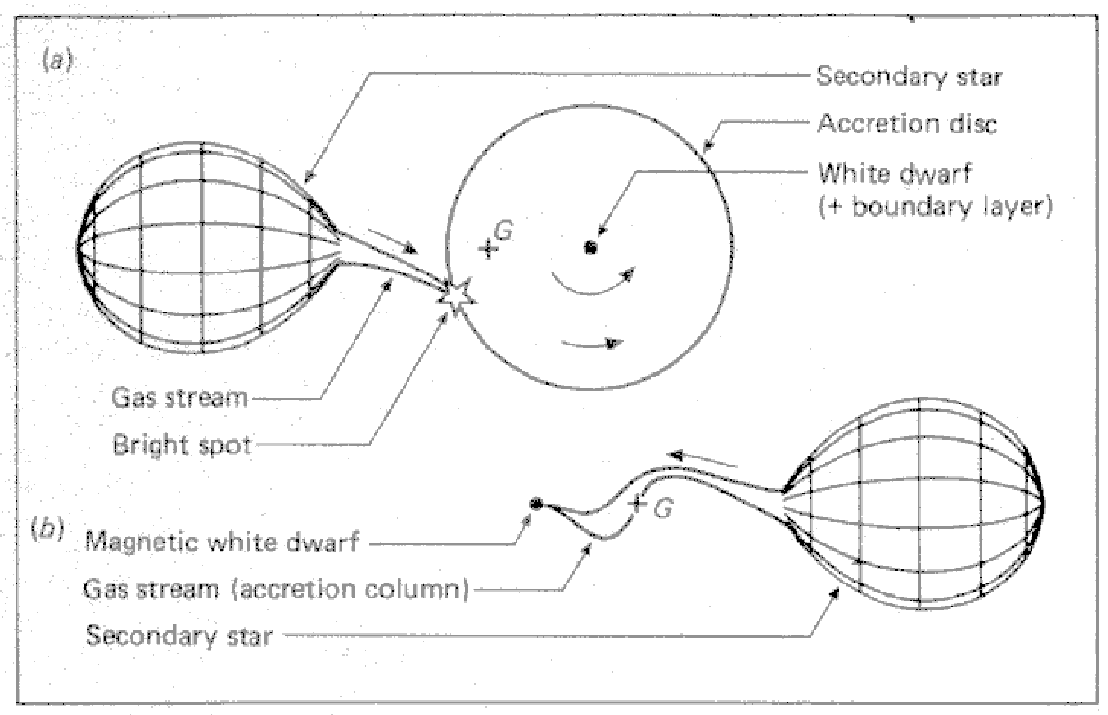
\includegraphics[scale=0.4]{Introduccion/Figures/Figura Acrecion_SmithReview.png}
	\caption{Diagrama de una estrella enana blanca absorbiendo material de su
		compañera estrella de secuencia principal por medio de la interacción de sus
		lóbulos de Roche.} \citet{smithReview}
	\label{acrecionSmithReview}
\end{figure}

Todas las variables cataclísmicas han obtenido su nombre debido a sus cambios
rápidos en sus propiedades durante periodos de observación. El mecanismo
principal que causa estas variaciones se debe a los estallidos periódicos,
conocidos como \textit{novae}. Al igual como no todos los sistemas muestran las
mismas propiedades en sus componentes existen diferentes tipos de estallidos:
\textit{novae clásicos}, \textit{novae enanos}, y \textit{nova-like}.
\cite*{smithReview} \\\newline
Los novae clásicos son aquellos estallidos observados en sistemas binarios que
causa que su luminosidad aumente por varias magnitudes en una escala de tiempo
relativamente corta (puede ser en la escala de días hasta meses).
\citet{smithReview} Aparte de la radiación generada debido a reacciones
termonucleares, los novae expulsan un entorno de gas caliente a grandes
velocidades, llegando a miles de kilómetros por segundo. Pocos sistemas binarios
muestran nova recurrentes a lo largo del tiempo en intervalos de decenas o
cientos de años; la mayoría ha mostrado un solo estallido en su tiempo de
observación. En sistemas no magnéticos, el disco de acreción sirve como el motor
principal de estos estallidos. La mayoría del material en el disco es hidrógeno;
este crea una capa en la superficie de la enana blanca. A lo largo de lo que se
acumula este material aumente su grosor, aumentando la temperatura de la capa.
Este aumento de temperatura causa que la presión en esta capa alcance un punto
en donde empiezan a ocurrir reacciones termonucleares de parte del hidrógeno
presente en esta capa.
}